\documentclass[spanish,a4paper,11pt,twoside]{report}

%%%%%%%%%%%%%%%%%%%%%%%%%%%%%%%%%%%%%%%%%%%%%%%%%%%%%%%%%%%%%%%%%%%%%%%%%%%%%%%
\usepackage[dvips]{graphicx}
\usepackage[dvips]{epsfig}
\usepackage[latin1]{inputenc}
\usepackage[spanish]{babel}
\usepackage{alltt}
%\usepackage{mem/templates/algorithm}
\usepackage{mem/templates/algorithmic}
\usepackage{mem/templates/multirow}

%%%%%%%%%%%%%%%%%%%%%%%%%%%%%%%%%%%%%%%%%%%%%%%%%%%%%%%%%%%%%%%%%%%%%%%%%%%%%%%

\newcommand{\SONY}{{\sc Sony}}
\newcommand{\MICROSOFT}{{\sc Microsoft}}
\newcommand{\GCC}{\textsf{\textsc{G}CC}}
\newcommand{\INTEL}{\textsf{\textsc{I}ntel}}

%%% Traducimos el pseudocodigo
\renewcommand{\algorithmicwhile}{\textbf{mientras}}
\renewcommand{\algorithmicend}{\textbf{fin}}
\renewcommand{\algorithmicdo}{\textbf{hacer}}
\renewcommand{\algorithmicif}{\textbf{si}}
\renewcommand{\algorithmicthen}{\textbf{entonces}}
\renewcommand{\algorithmicrepeat}{\textbf{repetir}}
\renewcommand{\algorithmicuntil}{\textbf{hasta que}}
\renewcommand{\algorithmicelse}{\textbf{en otro caso}}
\renewcommand{\algorithmicfor}{\textbf{para}}

%\newcommand{\RETURN}{\textbf{retornar} }
\newcommand{\RET}{\STATE \textbf{retornar} }
\newcommand{\TO}{\textbf{hasta} }
\newcommand{\AND}{\textbf{y} }
\newcommand{\OR}{\textbf{o} }

%%%%%%%%%%%%%%%%% Creamos un entorno para listar c�digo fuente %%%%%%%%%%%%%%%
\newenvironment{sourcecode}
{\begin{list}{}{\setlength{\leftmargin}{1em}}\item\scriptsize\bfseries}
{\end{list}}

\newenvironment{littlesourcecode}
{\begin{list}{}{\setlength{\leftmargin}{1em}}\item\tiny\bfseries}
{\end{list}}

\newenvironment{summary}
{\par\noindent\begin{center}\textbf{Abstract}\end{center}\begin{itshape}\par\noindent}
{\end{itshape}}

\newenvironment{keywords}
{\begin{list}{}{\setlength{\leftmargin}{1em}}\item[\hskip\labelsep \bfseries Keywords:]}
{\end{list}}

\newenvironment{palabrasClave}
{\begin{list}{}{\setlength{\leftmargin}{1em}}\item[\hskip\labelsep \bfseries Palabras clave:]}
{\end{list}}


%%%%%%%%%%%%%%%%%%%%%%%%%%%%%%%%%%%%%%%%%%%%%%%%%%%%%%%%%%%%%%%%%%%%%%%%%%%%%%%
% Format
%%%%%%%%%%%%%%%%%%%%%%%%%%%%%%%%%%%%%%%%%%%%%%%%%%%%%%%%%%%%%%%%%%%%%%%%%%%%%%%

%%\topmargin -4 mm
%\topmargin -21 mm
%\headheight 10 mm
%\headsep 10 mm

%\textheight 229 mm
%\textheight 246 mm

%\oddsidemargin -5.4 mm
%\evensidemargin -5.4 mm
\oddsidemargin 5 mm
\evensidemargin 5 mm

%\oddsidemargin -3 mm
%\evensidemargin -3 mm

%\textwidth 17 cm
\textwidth 15 cm
%\columnsep 10 mm

\input{amssym.def}

%%%%%%%%%%%%%%%%%%%%%%%%%%%%%%%%%%%%%%%%%%%%%%%%%%%%%%%%%%%%%%%%%%%%%%%%%%%%%%%

\begin{document}

%%%%%%%%%%%%%%%%%%%%%%%%%%%%%%%%%%%%%%%%%%%%%%%%%%%%%%%%%%%%%%%%%%%%%%%%%%%%%%%
% First Page 
%%%%%%%%%%%%%%%%%%%%%%%%%%%%%%%%%%%%%%%%%%%%%%%%%%%%%%%%%%%%%%%%%%%%%%%%%%%%%%%

\pagestyle{empty}
\thispagestyle{empty}


\newcommand{\HRule}{\rule{\linewidth}{1mm}}
\setlength{\parindent}{0mm}
\setlength{\parskip}{0mm}
\vspace*{\stretch{1}}

\begin{center}

\includegraphics[width=0.2\textwidth]{mem/images/logotipo-secundario-ULL}\\[0.25cm]
\end{center}

\HRule
\begin{center}
        {\Huge M�todo de Simpson} \\[2.5mm] 
        {\Huge Integraci�n num�rica} \\[2.5mm]
        {\Large Iv�n Trujillo Trujillo \\
        Samuel Santos Lucas Castilla} \\[5mm]
        {\Large \textit{Grupo 2J}} \\[5mm]


        {\em T�cnicas Experimentales. $1^{er}$ curso. $2^{do}$ semestre} \\[5mm]
        Lenguajes y Sistemas Inform�ticos \\[5mm]
        Facultad de Matem�ticas \\[5mm]
        
        Universidad de La Laguna \\
\end{center}
\HRule
\vspace*{\stretch{2}}
\begin{center}
  La Laguna, \today 
\end{center}

%%%%%%%%%%%%%%%%%%%%%%%%%%%%%%%%%%%%%%%%%%%%%%%%%%%%%%%%%%%%%%%%%%%%%%%%%%%%%%%

%%%%%%%%%%%%%%%%%%%%%%%%%%%%%%%%%%%%%%%%%%%%%%%%%%%%%%%%%%%%%%%%%%%%%%%%%%%%%%%
\newpage{\pagestyle{empty}\cleardoublepage}

\pagestyle{myheadings} %my head defined by markboth or markright
% No funciona bien \markboth sin "twoside" en \documentclass, pero al
% ponerlo se dan un mont�n de errores de underfull \vbox, con lo que no se
% ha puesto.
\markboth{Iv�n Trujillo y Samuel Lucas}{M�todo de Simpson}

%%%%%%%%%%%%%%%%%%%%%%%%%%%%%%%%%%%%%%%%%%%%%%%%%%%%%%%%%%%%%%%%%%%%%%%%%%%%%%%
%Numeracion en romanos
\renewcommand{\thepage}{\roman{page}}
\setcounter{page}{1}

%%%%%%%%%%%%%%%%%%%%%%%%%%%%%%%%%%%%%%%%%%%%%%%%%%%%%%%%%%%%%%%%%%%%%%%%%%%%%%%

\tableofcontents

%%%%%%%%%%%%%%%%%%%%%%%%%%%%%%%%%%%%%%%%%%%%%%%%%%%%%%%%%%%%%%%%%%%%%%%%%%%%%%%
\newpage{\pagestyle{empty}\cleardoublepage}

\listoffigures

%%%%%%%%%%%%%%%%%%%%%%%%%%%%%%%%%%%%%%%%%%%%%%%%%%%%%%%%%%%%%%%%%%%%%%%%%%%%%%%
\newpage{\pagestyle{empty}\cleardoublepage}

\listoftables

%%%%%%%%%%%%%%%%%%%%%%%%%%%%%%%%%%%%%%%%%%%%%%%%%%%%%%%%%%%%%%%%%%%%%%%%%%%%%%%
\newpage{\pagestyle{empty}\cleardoublepage}

%%%%%%%%%%%%%%%%%%%%%%%%%%%%%%%%%%%%%%%%%%%%%%%%%%%%%%%%%%%%%%%%%%%%%%%%%%%%%%%
%Numeracion a partir del capitulo I
\renewcommand{\thepage}{\arabic{page}}
\setcounter{page}{1}

\setlength{\parindent}{5mm}

%%%%%%%%%%%%%%%%%%%%%%%%%%%%%%%%%%%%%%%%%%%%%%%%%%%%%%%%%%%%%%%%%%%%%%%%%%%%%%%
\chapter{Motivaci�n y objetivos}
\label{chapter:obj}

%%%%%%%%%%%%%%%%%%%%%%%%%%%%%%%%%%%%%%%%%%%%%%%%%%%%%%%%%%%%%%%%%%%%%%%%%%%%%
% Chapter 1: Motivaci�n y Objetivos 
%%%%%%%%%%%%%%%%%%%%%%%%%%%%%%%%%%%%%%%%%%%%%%%%%%%%%%%%%%%%%%%%%%%%%%%%%%%%%%%

	El objetivo principal de este trabajo es implementar un programa en Python que sea capaz
de resolver el problema del c�lculo del �rea bajo una funci�n conocida en un intervalo cerrado.

	Para llevar a cabo este proyecto debemos hacer uso de la integraci�n num�rica utilizando el m�todo de 
Simpson, teniendo en cuenta los siguientes aspectos:
\begin{enumerate}
  \item Debemos comprender los conceptos b�sicos de la integraci�n aproximada empleando el m�todo de Simpson.
  \item Debemos valorar el error producido entre el valor real y la aproximaci�n obtenida.
  \item Debemos analizar las representaciones gr�ficas de la funci�n estudiada y de la par�bola hallada por el m�todo de Simpson.
\end{enumerate}

%---------------------------------------------------------------------------------
\section{Objetivos espec�ficos}
\label{1:sec:1}
	Se realizar� el experimento con una funci�n conocida y definida en intervalos cerrados.
	
La funci�n dada es: 

\[f(x) = \frac{1}{1+e^{x}}, \quad x \in [1, 6]\]





%%%%%%%%%%%%%%%%%%%%%%%%%%%%%%%%%%%%%%%%%%%%%%%%%%%%%%%%%%%%%%%%%%%%%%%%%%%%%%%
\chapter{Fundamentos te�ricos}
\label{chapter:teo}


%%%%%%%%%%%%%%%%%%%%%%%%%%%%%%%%%%%%%%%%%%%%%%%%%%%%%%%%%%%%%%%%%%%%%%%%%%%%%%%
% Chapter 2: Fundamentos Te�ricos 
%%%%%%%%%%%%%%%%%%%%%%%%%%%%%%%%%%%%%%%%%%%%%%%%%%%%%%%%%%%%%%%%%%%%%%%%%%%%%%%

%++++++++++++++++++++++++++++++++++++++++++++++++++++++++++++++++++++++++++++++

Podemos decir que uno de los problemas m�s frecuentes en las matem�ticas es el c�lculo del �rea que obtiene a 
apartir de una funcion f(x), el eje x y los l�mites a y b.Por ejemplo, queremos calcular el �rea de la figura 1, 
recaslcando que dicha �rea est� comprendido entre los l�mites a y b, y por debajo de la funcion f(x):
 
 %aqui va el includegrafic de la fichura 1

Partiendo de que conocemos la funci�n y los valores de a y b: b lo consideramos como el l�mite superior y a como 
el l�mite inferior. Podemos obtener dos tipos de soluciones:

\begin{itemize}
\item Soluciones algebraicas: obtenemos una f�rmula exacta y precisa del �rea solicitada.
\item Soluciones num�ricas: calculamos de manera num�rica una estimaci�n o aproximacion del �rea.
\end{itemize}

Respecto a estos tipos de soluciones sabemos de antemano que las solcuiones algebraicas son mejores que las num�ricas, dado que son exactas. Pero se da el caso de que a veces, la complejidad de las funciones hace dif�cil la obtenci�n de la solcui�n algebraica, por lo que la solci�n num�rica nos permite ahorrar tiempo. Como ejemplo de esta aproximaci�n tenemos el M�todo de Simpson:

%++++++++++++++++++++++++++++++++++++++++++++++++++++++++++++++++++++++++++++++

\section{Primer apartado del segundo cap�tulo}
\label{2:sec:1}
  Primer p�rrafo de la primera secci�n.

\section{Segundo apartado del segundo cap�tulo}
\label{2:sec:2}
  Primer p�rrafo de la segunda secci�n.




%%%%%%%%%%%%%%%%%%%%%%%%%%%%%%%%%%%%%%%%%%%%%%%%%%%%%%%%%%%%%%%%%%%%%%%%%%%%%%%
\chapter{Procedimiento experimental}
\label{chapter:exp}

%%%%%%%%%%%%%%%%%%%%%%%%%%%%%%%%%%%%%%%%%%%%%%%%%%%%%%%%%%%%%%%%%%%%%%%%%%%%%%%
% Chapter 3: Procedimiento experimental 
%%%%%%%%%%%%%%%%%%%%%%%%%%%%%%%%%%%%%%%%%%%%%%%%%%%%%%%%%%%%%%%%%%%%%%%%%%%%%%%

	A continuaci�n se proceder� a describir detalladamente el experimento llevado a cabo.
Se hablar� de en qu� consiste exactamente, en qu� se basa y como se ha planteado su
resoluci�n. Seguidamente, se enumerar� el material necesario para realizar la prueba.
Otro apartado estar� dedicado a mencionar los resultados que se han obtenido sin realizar
ninguna objeci�n sobre la implicaci�n de los mismos. Por �ltimo, se har� uso de los
conocimientos expuestos en el cap�tulo 2 para poder analizar los datos que hemos
obtenido y, as� mismo, lo que ello supone.

%++++++++++++++++++++++++++++++++++++++++++++++++++++++++++++++++++++++++++++++
\section{Descripci�n de los experimentos}
\label{3:sec:1}
	 Para la realizaci�n del experimento se ha utilizado b�sicamente un editor de texto
para escribir el c�digo fuente de Python y un int�rprete del mismo. El experimento consiste
en la realizaci�n de un programa en Python que sea capaz de calcular el valor de una integral
definida en un intervalo cerrado, que a su vez calcule su aproximaci�n por el m�todo de Simpson,
halle los errores relativo y absoluto entre los dos valores obtenidos y realice la representaci�n
gr�fica de la funci�n que se desea integrar y la par�bola generada por el m�todo utilizado
para su aproximaci�n. Como hemos mencionado anteriormente, se ha trabajado con una
funci�n dada ($f(x) = \frac{1}{1+e^{x}}$) definida en el intervalo $x \in [1, 6]$.

	Hay que considerar que la integral de f es $f'(x) = \ln{e^{x}} - \ln({e^{x}+1)}$ para poder
resolver la integral y hallar el valor real del �rea. Tambi�n debemos saber que la par�bola
que se ha de representar est� formada por los puntos f(a),f(b) y f($\frac{a+b}{2}$), por
lo que la ecuaci�n es $y = 0.0169x^2 - 0.17x + 0.422 $. 

%++++++++++++++++++++++++++++++++++++++++++++++++++++++++++++++++++++++++++++++
\section{Descripci�n del material}
\label{3:sec:2}
	En cuesti�n al material empleado para realizar el experimento se ha utilizado un
computador con un procesador Intel(R) Core(TM)2 Quad CPU Q6600 @ 2.40GHz 2.39 GHz y 
una memoria RAM de 3,00 GB. El sistema operativo que conten�a el computador era 
Windows 7 Home Premium de 32 bits. Para escribir los c�digos fuente de LaTeX se
usaron los programas Texmaker y Kate (versiones 3.2 y 3.8.5, respectivamente) y para 
el c�digo fuente de Python solamente se utiliz� Kate. Adem�s, para registrar los cambios
realizados en el trabajo y subirlos a GitHub se hizo uso de Git (1.7.9.5). Como 
compiladores se emple� el int�rprete de Python y el compilador de Tex.

%++++++++++++++++++++++++++++++++++++++++++++++++++++++++++++++++++++++++++++++
\section{Resultados obtenidos}
\label{3:sec:3}

bla, bla, etc. 

%------------------------------------------------------------------------------
%--------------------------------------------------------------------------
\begin{table}[!ht]
\begin{center}
\begin{tabular}{|c|c|} \hline 
\textbf{Tiempo  } & \textbf{Velocidad} \\ 
\textbf{($\pm$ 0.001 s)} & \textbf{($\pm$ 0.1 m/s)} \\ \hline \hline
1.234 &
67.8
\\
\hline

2.345 &
78.9
\\
\hline

3.456 &
89.1
\\
\hline

4.567 &
91.2
\\
\hline

\end{tabular}
\end{center}
\caption{Resultados experimentales de tiempo (s) y velocidad (m/s)}
\label{tab:1}
\end{table}


%------------------------------------------------------------------------------

%------------------------------------------------------------------------------
%\begin{figure}[!th]
\begin{center}
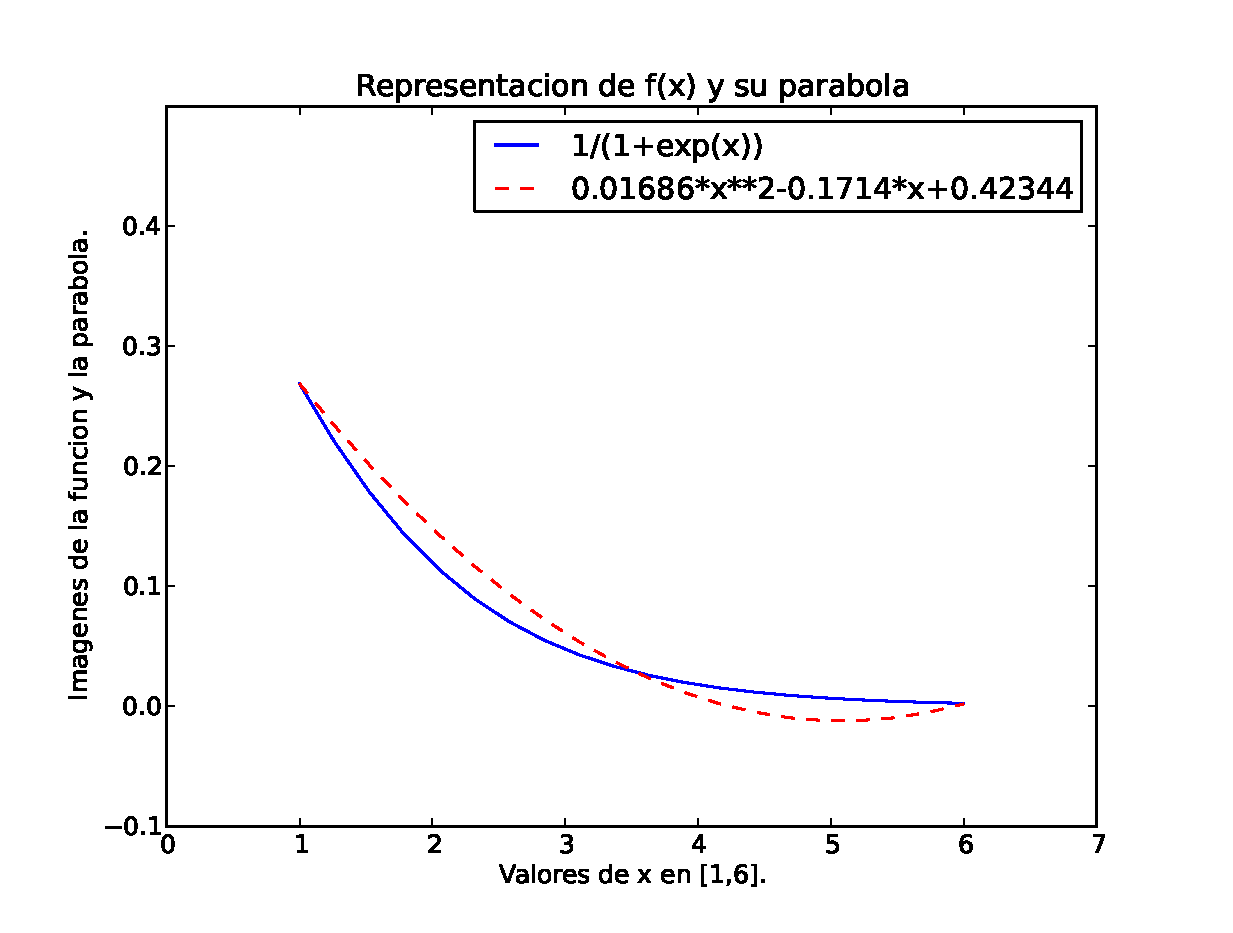
\includegraphics[width=0.85\textwidth]{mem/images/rep_funcion.eps}
%\caption{Gr�fica de la funci�n y su par�bola}
\label{fig:1}
\end{center}
%\end{figure}
%------------------------------------------------------------------------------

%++++++++++++++++++++++++++++++++++++++++++++++++++++++++++++++++++++++++++++++
\section{An�lisis de los resultados}
\label{3:sec:4}

bla, bla, etc. 



%%%%%%%%%%%%%%%%%%%%%%%%%%%%%%%%%%%%%%%%%%%%%%%%%%%%%%%%%%%%%%%%%%%%%%%%%%%%%%%
\chapter{Conclusiones}
\label{chapter:conclusiones}

%%%%%%%%%%%%%%%%%%%%%%%%%%%%%%%%%%%%%%%%%%%%%%%%%%%%%%%%%%%%%%%%%%%%%%%%%%%%%
% Chapter 4: Conclusiones y Trabajos Futuros 
%%%%%%%%%%%%%%%%%%%%%%%%%%%%%%%%%%%%%%%%%%%%%%%%%%%%%%%%%%%%%%%%%%%%%%%%%%%%%%%

\begin{itemize}

	\item El m\'etodo de Simpson es muy \'util para funciones con una curva similar a una par\'abola en un intervalo cerrado.

	\item El m\'etodo de Simpson produce una mala aproximaci\'on si la funci\'on en el intervalo cerrado presenta una recta o m\'as de una curva.
	
	\item El m\'etodo de Simpson facilita en gran medida la integraci\'on de funciones muy dif\'iciles de resolver por otros m\'etodos.

	\item El m\'etodo de Simpson es f\'acil de aplicar ya que solo hace falta utilizar una f\'ormula y hallar las im\'agenes de la funci\'on en tres puntos diferentes.
	
	\item El m\'etodo de Simpson puede ser utilizado para comprobar el resultado de una integraci\'on y sabemos que el error es m\'inimo.
	
	\item El m\'etodo de Simpson es algo complicado de demostrar si no se tienen ciertos conocimientos matem\'aticos, por eso suele ser un m\'etodo m\'as sistem\'atico.

\end{itemize}


%%%%%%%%%%%%%%%%%%%%%%%%%%%%%%%%%%%%%%%%%%%%%%%%%%%%%%%%%%%%%%%%%%%%%%%%%%%%%%%

%%%%%%%%%%%%%%%%%%%%%%%%%%%%%%%%%%%%%%%%%%%%%%%%%%%%%%%%%%%%%%%%%%%%%%%%%%%%%%%
\newpage{\pagestyle{empty}\cleardoublepage}
\thispagestyle{empty}
\begin{appendix}

\chapter{T�tulo del Ap�ndice 1}
\label{appendix:1}

\section{Algoritmo XXX}
\label{Apendice1:XXX}

\begin{center}
\begin{footnotesize}
\begin{verbatim}
###################################################################################
# Fichero .py
###################################################################################
#
# AUTORES
#   
# FECHA
#
# DESCRIPCION
#
###################################################################################
\end{verbatim}
\end{footnotesize}
\end{center}

\section{Algoritmo YYY}
\label{Apendice1:YYY}

\begin{center}
\begin{footnotesize}
\begin{verbatim}
/###################################################################################
 # Fichero .h
 ###################################################################################
 #
 # AUTORES
 #
 # FECHA
 #
 # DESCRIPCION
 #
 ##################################################################################
\end{verbatim}
\end{footnotesize}
\end{center}


\chapter{T�tulo del Ap�ndice 2}
\label{appendix:2}

\section{Otro apendice: Seccion 1}
\label{Apendice2:label}

\begin{center}
\begin{footnotesize}

\begin{verbatim}
Texto
\end{verbatim}

\end{footnotesize}
\end{center}

\section{Otro apendice: Seccion 2}
\label{Apendice2:label2}

\begin{center}
\begin{footnotesize}

\begin{verbatim}
Texto
\end{verbatim}


\end{footnotesize}
\end{center}


\end{appendix}

%%%%%%%%%%%%%%%%%%%%%%%%%%%%%%%%%%%%%%%%%%%%%%%%%%%%%%%%%%%%%%%%%%%%%%%%%%%%%%%
\addcontentsline{toc}{chapter}{Bibliograf�a}
\bibliographystyle{plain}


\bibliography{mem/bib/references}
\nocite{*}

%%%%%%%%%%%%%%%%%%%%%%%%%%%%%%%%%%%%%%%%%%%%%%%%%%%%%%%%%%%%%%%%%%%%%%%%%%%%%%%

\end{document}
